% Step and impulse response of a P-Glied (G(s) = K_p)
% Left: step response h(t) = K_p * sigma(t)
% Right: impulse response g(t) = K_p * delta(t) (visualised as a unit-area arrow)

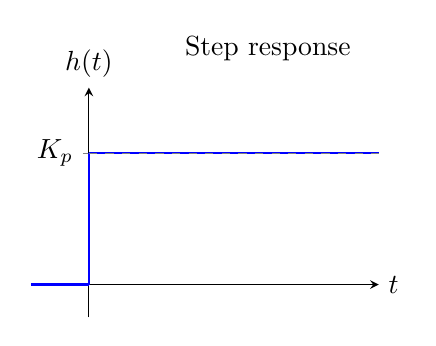
\begin{tikzpicture}
    \begin{axis}[
        width=6cm, height=4.5cm,
        xlabel={$t$}, ylabel={$h(t)$},
        title={Step response},
        title style={xshift=8mm},
        axis lines=middle,
        xmin=-1, xmax=5,
        ymin=-0.5, ymax=3,
        xtick=\empty, ytick={2},
        yticklabels={$K_p$},
        every axis y label/.style={at={(ticklabel* cs:1.0)}, anchor=south},
        every axis x label/.style={at={(ticklabel* cs:1.0)}, anchor=west},
        clip=false
    ]
        \addplot[blue, thick, domain=-1:0, samples=2] {0};
        \addplot[blue, thick, domain=0:5, samples=2] {2};
        \draw[blue, thick] (axis cs:0,0) -- (axis cs:0,2);
        \draw[dashed, gray] (axis cs:0,2) -- (axis cs:5,2);
    \end{axis}
\end{tikzpicture}%
\hspace{0.6cm}%
\begin{tikzpicture}
    \begin{axis}[
        width=6cm, height=4.5cm,
        xlabel={$t$}, ylabel={$g(t)$},
        title={Impulse response},
        title style={xshift=8mm},
        axis lines=middle,
        xmin=-1, xmax=5,
        ymin=-0.5, ymax=3,
        xtick=\empty, ytick=\empty,
        every axis y label/.style={at={(ticklabel* cs:1.0)}, anchor=south},
        every axis x label/.style={at={(ticklabel* cs:1.0)}, anchor=west},
        clip=false
    ]
        \addplot[orange, thick, domain=-1:5, samples=2] {0};
        \draw[orange, thick, -{Latex[length=3mm]}] (axis cs:0,0) -- (axis cs:0,2.5);
        \node[orange, anchor=west] at (axis cs:0.15,2.2) {$K_p \cdot \delta(t)$};
    \end{axis}
\end{tikzpicture}
